\documentclass[12pt, a4paper]{report}

\usepackage{graphicx}

% ── Encoding & language
\usepackage[utf8]{inputenc}
\usepackage[T1]{fontenc}
\usepackage[french]{babel}

% ── Typography ────────────────────────────────────────────────────────────────
\usepackage{lmodern}
\usepackage{microtype}
\usepackage{setspace}
\onehalfspacing

% ── Page geometry ─────────────────────────────────────────────────────────────
\usepackage[top=2.5cm, bottom=2.5cm, left=3cm, right=3cm]{geometry}

% ── Maths ─────────────────────────────────────────────────────────────────────
\usepackage{amsmath, amssymb}

% ── Hyperlinks ────────────────────────────────────────────────────────────────
\usepackage[hidelinks]{hyperref}

% ── Syntax highlighting (minted) ──────────────────────────────────────────────
% pip install Pygments  then compile with:  pdflatex --shell-escape report.tex
\usepackage{minted}
\setminted{
  fontsize=\small,
  linenos=true,
  breaklines=true,
  frame=lines,
  framesep=4pt,
  bgcolor=gray!3,
  numbersep=8pt,
  style=emacs,
}

% ── Headers / footers ─────────────────────────────────────────────────────────
\usepackage{fancyhdr}
\pagestyle{fancy}
\fancyhf{}
\fancyhead[L]{\leftmark}
\fancyhead[R]{\thepage}
\renewcommand{\headrulewidth}{0.4pt}

% =============================================================================
\begin{document}

% ── Title page ────────────────────────────────────────────────────────────────
\begin{titlepage}
  \centering
  \vspace*{3cm}

  {\Huge\bfseries  Impl\'ementation, optimisation et diffusion d’algorithmes d’unranking\par}
  \vspace{3cm}

  {\Large\itshape Nouriddin Boukhzar \& Ayoub Salhi\par}
  {\large Encadrant: Amaury Curiel\par}
  \vspace{1cm}
  {\normalsize Sorbonne universit\'e\par}
\end{titlepage}

% ── Table of contents ─────────────────────────────────────────────────────────
\tableofcontents
\clearpage

% =============================================================================
\chapter{Introduction}

Dans les ann\'ees 1960, le math\'ematicien Gian-Carlo Rota a identifi\'e 12
probl\`emes fondamentaux en combinatoire. Si les formules de comptage associ\'ees
\`a ces probl\`emes sont connues depuis longtemps, ce n'est que r\'ecemment que
des algorithmes permettant de g\'en\'erer chacune de ces structures de mani\`ere
syst\'ematique ont \'et\'e propos\'es.

Ce projet a pour objectif d'impl\'ementer ces algorithmes, de les optimiser via la
programmation concurrente, puis de les int\'egrer \`a la biblioth\`eque Python
SymPy, r\'ef\'erence en calcul symbolique. En parall\`ele, une application web
sera d\'evelopp\'ee afin de rendre ces algorithmes accessibles et visualisables
en ligne.

% =============================================================================
\chapter{T\^aches \`a r\'ealiser}

\section{Algorithmes d'unranking}

La premi\`ere t\^ache consiste \`a impl\'ementer les algorithmes d'unranking
pour chacun des 12 probl\`emes de Rota. Ces algorithmes permettent, \`a partir
d'un entier, de retrouver directement la structure combinatoire associ\'ee sans
\'enum\'erer toutes les structures pr\'ec\'edentes.

\section{Application web}

Dans le m\^eme temps, une application web sera d\'evelopp\'ee pour permettre
d'ex\'ecuter ces algorithmes en ligne et d'en visualiser le fonctionnement.
L'objectif est de rendre ces outils accessibles sans n\'ecessiter d'installation
locale.

\section{Contribution \`a SymPy}

Enfin, les algorithmes impl\'ement\'es seront adapt\'es aux standards de la
biblioth\`eque open-source SymPy, afin d'y \^etre int\'egr\'es et mis \`a
disposition de la communaut\'e. Cette \'etape implique de respecter les conventions
de code, de documentation et de tests propres au projet.

% =============================================================================
\chapter{Les algorithmes (ordre combinatoire)}

\section{Partitions de Stirling}

\subsection{Formule de comptage}

Le nombre de partitions de Stirling de $\{1, \ldots, n\}$ en $k$ blocs est donn\'e
par les nombres de Stirling de seconde esp\`ece, not\'es $\left\{n \atop k\right\}$,
d\'efinis par la r\'ecurrence suivante :

\[
  \left\{n \atop k\right\} =
  \begin{cases}
    1 & \text{si } k = 1 \text{ ou } k = n \\[6pt]
    \left\{n-1 \atop k-1\right\} + k \cdot \left\{n-1 \atop k\right\}
      & \text{sinon}
  \end{cases}
\]

\subsection{Interpr\'etation combinatoire}

Cette r\'ecurrence se comprend naturellement : pour construire une $k$-partition
de $\{1, \ldots, n\}$, on consid\`ere le placement de l'\'el\'ement $n$. Soit on
cr\'ee un nouveau bloc singleton $\{n\}$, en compl\'etant une $(k-1)$-partition
de $\{1, \ldots, n-1\}$, ce qui donne $\left\{n-1 \atop k-1\right\}$
possibilit\'es, soit on ins\`ere $n$ dans l'un des $k$ blocs d'une $k$-partition
existante de $\{1, \ldots, n-1\}$, ce qui donne
$k \cdot \left\{n-1 \atop k\right\}$ possibilit\'es.

\subsection{Impl\'ementation}

L'algorithme d'unranking suit directement cette d\'ecomposition. \'Etant donn\'e
un rang $r$, on d\'etermine si $n$ forme un bloc singleton (cas~A) ou s'il est
ins\'er\'e dans un bloc existant (cas~B), en comparant $r$ au nombre de partitions
du cas~A. Dans le second cas, une division euclidienne permet d'identifier le bloc
cible et le rang r\'esiduel pour l'appel r\'ecursif.

Les nombres de Stirling pouvant devenir tr\`es grands, ils sont repr\'esent\'es en
\texttt{bigint}. Un cache LRU est utilis\'e pour \'eviter de recalculer les
m\^emes valeurs lors des appels r\'ecursifs.

\begin{minted}{typescript}
const stirling_numbers_cache = new LRUCache<string, bigint>({max: 5000});
function stirling_numbers(n: bigint, k: bigint): bigint {
  // There is exactly 1 way to partition 0 elements into 0 groups.
  if (n == 0 && k == 0) return 1;
  // ex: Partition 0 elements into 3 groups -> impossible
  if (n == 0 || k == 0) return 0;
  const s = serialize_nk(n, k);
  const cached = stirling_numbers_cache.get(s);
  if (cached !== undefined) return cached;
  const res = stirling_numbers(n-1, k-1) + k*stirling_numbers(n-1, k);
  stirling_numbers_cache.set(s, res);
  return res;
}
function unrank_stirling(n, k, r): number[][] {
  if (n == 0 || k == 0)
    return [];
  const cntA = stirling_numbers(n-1, k-1);
  if (r < cntA) {
    let res = unrank_stirling(n-1, k-1, r);
    res.push([n]);
    return res
  }
  const r2 = r - cntA;
  const [pos, r3] = divmod(r2, stirling_numbers(n-1, k));
  let us = unrank_stirling(n-1, k, r3);
  us[pos].push(n);
  return us;
}
\end{minted}

\section{Partitions de Stirling Ordonn\'ees}

\subsection{Formule de comptage}

Le nombre de partitions de Stirling ordonn\'ees de $\{1, \ldots, n\}$ en $k$ blocs
est not\'e $O^n_k$ et satisfait la r\'ecurrence suivante :

\[
  O^n_k =
  \begin{cases}
    k! & \text{si } k = 1 \text{ ou } k = n \\[6pt]
    k \cdot (O^{n-1}_{k-1} + O^{n-1}_k) & \text{sinon}
  \end{cases}
\]

\subsection{Interpr\'etation combinatoire}

Une partition de Stirling ordonn\'ee est une partition de Stirling dont les blocs
sont ordonn\'es. La r\'ecurrence se comprend comme suit : pour construire une
$k$-partition de $\{1, \ldots, n\}$, soit on ajoute $n$ comme nouveau bloc singleton
dans l'une des $k$ positions possibles parmi les blocs existants d'une
$(k-1)$-partition de $\{1, \ldots, n-1\}$, soit on ins\`ere $n$ dans l'un des $k$
blocs d'une $k$-partition existante de $\{1, \ldots, n-1\}$. Dans les deux cas, on
multiplie par $k$, d'o\`u la relation $O^n_k = k \cdot (O^{n-1}_{k-1} + O^{n-1}_k)$.

Aux cas de base, si $k = 1$ tous les \'el\'ements sont dans un seul bloc et il n'y
a qu'une seule partition. Si $k = n$ chaque \'el\'ement est dans son propre bloc, et
toute permutation de ces blocs donne une partition diff\'erente, soit $k!$ partitions.

\subsection{Impl\'ementation}

L'algorithme d'unranking suit la m\^eme logique que pour les partitions de Stirling
classiques, \`a ceci pr\`es que l'ordre des blocs est significatif. \'Etant donn\'e
un rang $r$, on d\'etermine d'abord si $n$ forme un nouveau bloc singleton (cas~A),
en comparant $r$ \`a $k \cdot O^{n-1}_{k-1}$. Dans ce cas, une division euclidienne
identifie la position du nouveau bloc. Sinon (cas~B), $n$ est ins\'er\'e dans un bloc
existant, et une seconde division euclidienne d\'etermine lequel.

\begin{minted}{typescript}
const ordered_stirling_cache = new LRUCache<string, number>({max: 5000});
function ordered_stirling_numbers(n, k): bigint {
  const key = serialize_nk(n, k);
  const cached = ordered_stirling_cache.get(key);
  if (cached !== undefined) return cached;
  if (k === 1 || k === n) {
    const result = factorial(k);
    ordered_stirling_cache.set(key, result);
    return result;
  }
  const result = k * (ordered_stirling_numbers(n - 1, k - 1) +
    ordered_stirling_numbers(n - 1, k));
  ordered_stirling_cache.set(key, result);
  return result;
}
function unrank_ordered_stirling(n, k, r) {
  if (k === 1)
    return [Array.from({ length: n }, (_, i) => i + 1)];
  if (k === n) {
    let perm = unrank_perm(n, r);
    return perm.map(x => [x]);
  }
  // Case A: n is put in a singleton, which is inserted in position `pos`
  let cntA = k * ordered_stirling_numbers(n - 1, k - 1);
  if (r < cntA) {
    let [pos, newR] = divmod(r, ordered_stirling_numbers(n - 1, k - 1));
    let res = unrank_ordered_stirling(n - 1, k - 1, newR);
    res.splice(pos, 0, [n]);
    return res;
  }
  // Case B: n is put in an existing block
  r = r - cntA;
  let [pos, newR] = divmod(r, ordered_stirling_numbers(n - 1, k));
  let res = unrank_ordered_stirling(n - 1, k, newR);
  res[pos].push(n);
  return res;
}
\end{minted}

\section{Partitions de Lah}

\subsection{Formule de comptage}

Le nombre de partitions de Lah de $\{1, \ldots, n\}$ en $k$ blocs est donn\'e par
les nombres de Lah, not\'es $\left\lfloor n \atop k \right\rfloor$, d\'efinis par
la r\'ecurrence suivante :

\[
  \left\lfloor n \atop k \right\rfloor =
  \begin{cases}
    n! & \text{si } k = 1 \\[6pt]
    1  & \text{si } k = n \\[6pt]
    \left\lfloor n-1 \atop k-1 \right\rfloor + (n - 1 + k) \cdot
    \left\lfloor n-1 \atop k \right\rfloor & \text{sinon}
  \end{cases}
\]

\subsection{Interpr\'etation combinatoire}

Une partition de Lah est une partition dont les blocs sont des s\'equences ordonn\'ees,
mais dont l'ensemble des blocs est lui-m\^eme non ordonn\'e. Autrement dit, l'ordre
des \'el\'ements \textit{au sein} de chaque bloc compte, mais l'ordre des blocs entre
eux ne compte pas.

La r\'ecurrence se comprend comme suit : pour construire une $k$-partition de
$\{1, \ldots, n\}$, soit on ajoute $n$ comme nouveau bloc singleton, en compl\'etant
une $(k-1)$-partition de $\{1, \ldots, n-1\}$, soit on ins\`ere $n$ dans l'un des
$k$ blocs existants d'une $k$-partition de $\{1, \ldots, n-1\}$. Dans ce dernier
cas, $n$ peut \^etre plac\'e en t\^ete ou apr\`es n'importe lequel des $n - 1$
\'el\'ements d\'ej\`a pr\'esents, r\'epartis dans $k$ blocs, ce qui donne $n - 1 + k$
positions possibles.

Aux cas de base, si $k = 1$ tous les \'el\'ements forment une seule s\'equence, soit
$n!$ arrangements possibles. Si $k = n$ chaque \'el\'ement est seul dans son bloc,
et il n'existe qu'une seule telle partition.

\subsection{Impl\'ementation}

L'algorithme d'unranking suit cette d\'ecomposition. \'Etant donn\'e un rang $r$,
on compare $r$ au nombre de partitions du cas singleton (cas~A). Si $r$ est inf\'erieur,
$n$ forme un nouveau bloc et on r\'ecure sur une $(k-1)$-partition de $\{1,\ldots,n-1\}$.
Sinon (cas~B), une division euclidienne identifie le bloc cible, puis on parcourt les
blocs pour localiser la position d'insertion exacte de $n$.

\begin{minted}{typescript}
const lah_numbers_cache = new LRUCache<string, bigint>({max: 5000});

function lah_numbers(n: bigint, k: bigint): bigint {
  if (n == 0 && k == 0) return 1;
  if (n == 0 || k == 0) return 0;
  if (n == k) return 1;

  const key = serialize_nk(n, k);

  const cached = lah_numbers_cache.get(key);
  if (cached !== undefined) return cached;

  const res = lah_numbers(n-1, k-1) + (n+k-1)*lah_numbers(n-1, k);
  lah_numbers_cache.set(key, res);
  return res;
}

function unrank_lah(n, k, r) {
  if (n == 0 && k == 0) return [];
  if (n == 0 || k == 0) return [];
  if (n == k)
    return Array.from({ length: n }, (_, x) => [x + 1]);

  // Case A: create a singleton with n
  let fst_case_cnt = lah_numbers(n-1, k-1);
  if (r < fst_case_cnt)
    return [...unrank_lah(n-1, k-1, r), [n]];

  // Case B: n is inserted in an existing block
  const r2 = r - fst_case_cnt;
  let [pos, r3] = divmod(r2, lah_numbers(n-1, k));
  let res = unrank_lah(n-1, k, r3);

  for (const boite of res) {
    if (pos < boite.length + 1) {
      boite.splice(pos, 0, n);
      break;
    }
    pos -= boite.length + 1;
  }
  return res;
}
\end{minted}

\section{Partitions Enti\`eres}

\subsection{Formule de comptage}

Le nombre de partitions de l'entier $n$ en $k$ parts est not\'e $p(n, k)$ et
satisfait la r\'ecurrence suivante :

\[
  p(n, k) =
  \begin{cases}
    0 & \text{si } n < 1 \\[6pt]
    1 & \text{si } k = 1 \text{ ou } k = n \\[6pt]
    p(n-1, k-1) + p(n-k, k) & \text{sinon}
  \end{cases}
\]

\subsection{Interpr\'etation combinatoire}

Une partition enti\`ere de $n$ en $k$ parts est un multiensemble de $k$ entiers
strictement positifs dont la somme vaut $n$. Contrairement aux partitions d'ensembles
vues pr\'ec\'edemment, il n'y a pas d'\'el\'ements \`a distribuer : on d\'ecompose
un entier en parts.

La r\'ecurrence se comprend comme suit : pour construire une $k$-partition de $n$,
soit la plus petite part vaut $1$, et il reste \`a partitionner $n - 1$ en $k - 1$
parts, soit toutes les parts sont strictement sup\'erieures \`a $1$, auquel cas on
peut soustraire $1$ \`a chacune des $k$ parts, ce qui ram\`ene au probl\`eme de
partitionner $n - k$ en $k$ parts.

Aux cas de base, si $k = 1$ la seule partition possible est $\{n\}$, et si $k = n$
la seule partition possible est $\{1, 1, \ldots, 1\}$.

\subsection{Impl\'ementation}

L'algorithme d'unranking suit directement cette d\'ecomposition. \'Etant donn\'e
un rang $r$, on compare $r$ au nombre de partitions dont la plus petite part vaut
$1$ (cas~A). Si $r$ est inf\'erieur, on place un $1$ en tête et on r\'ecure sur
une $(k-1)$-partition de $n-1$. Sinon (cas~B), on r\'ecure sur une $k$-partition
de $n - k$ et on ajoute $1$ \`a chaque part du r\'esultat.

\begin{minted}{typescript}
export function unrank_int_partitions(n, k, r) {
  if (n < 1) return [];
  if (k === 1) return [n];
  if (n === k) return Array(n).fill(1);

  // Case A: smallest part is 1
  const partitionsCount = int_partitions(n - 1, k - 1);
  if (r < partitionsCount)
    return [1, ...unrank_int_partitions(n - 1, k - 1, r)];

  // Case B: all parts are > 1, subtract 1 from each
  const r2 = r - partitionsCount;
  const res = unrank_int_partitions(n - k, k, r2);
  return res.map(i => i + 1);
}
\end{minted}

\chapter{Application Web}

\section{Fonctionnement}

L'application doit permettre d'ex\'ecuter les algorithmes d'unranking directement
depuis un navigateur, sans installation locale ni serveur de calcul. Cela impose
que l'ensemble de la logique algorithmique s'ex\'ecute c\^ot\'e client. Par
ailleurs, certains calculs peuvent \^etre longs pour de grandes valeurs de $n$ et
$k$, ce qui soul\`eve la question de la r\'eactivit\'e de l'interface.

\section{Justification des choix techniques}

\subsection{React + Vite + TypeScript}

L'application est d\'evelopp\'ee avec React, Vite et TypeScript. React permet de
structurer l'interface de mani\`ere claire et r\'eactive. Vite offre un
environnement de d\'eveloppement rapide et une cha\^ine de compilation moderne.
TypeScript apporte la s\^uret\'e des types, particuli\`erement utile pour
manipuler des \texttt{bigint} et des structures combinatoires potentiellement
complexes.

\subsection{Ex\'ecution dans un Web Worker}

Les algorithmes d'unranking sont ex\'ecut\'es dans un \textit{Web Worker}, c'est-\`a-dire
un thread s\'epar\'e du thread principal du navigateur. Cela pr\'esente plusieurs
avantages :

\begin{itemize}
  \item L'interface reste r\'eactive pendant le calcul — l'utilisateur peut
        toujours interagir avec la page.
  \item Les calculs lourds ne bloquent pas le rendu visuel.
\end{itemize}

En contrepartie, cette approche implique quelques limitations :

\begin{itemize}
  \item La communication entre le thread principal et le worker se fait par
        \'echange de messages, ce qui introduit une l\'eg\`ere latence.
  \item Le worker ne peut pas acc\'eder directement au DOM.
  \item En cas de calcul trop long, il n'est pas possible d'interrompre
        proprement le thread depuis l'ext\'erieur : la seule solution est de
        le terminer enti\`erement.
\end{itemize}

C'est ce dernier point qui a motiv\'e l'ajout d'un bouton \textbf{Abort} :
lorsqu'un calcul semble bloquer, l'utilisateur peut terminer le worker en cours
et en recr\'eer un nouveau imm\'ediatement, ce qui restitue le contr\^ole sans
avoir \`a recharger la page.

\section{Pr\'esentation}

L'interface se compose d'un formulaire permettant de saisir les param\`etres
$n$, $k$ et $r$, de s\'electionner l'algorithme souhait\'e, et de lancer
diff\'erentes actions.

\begin{figure}[h]
  \centering
  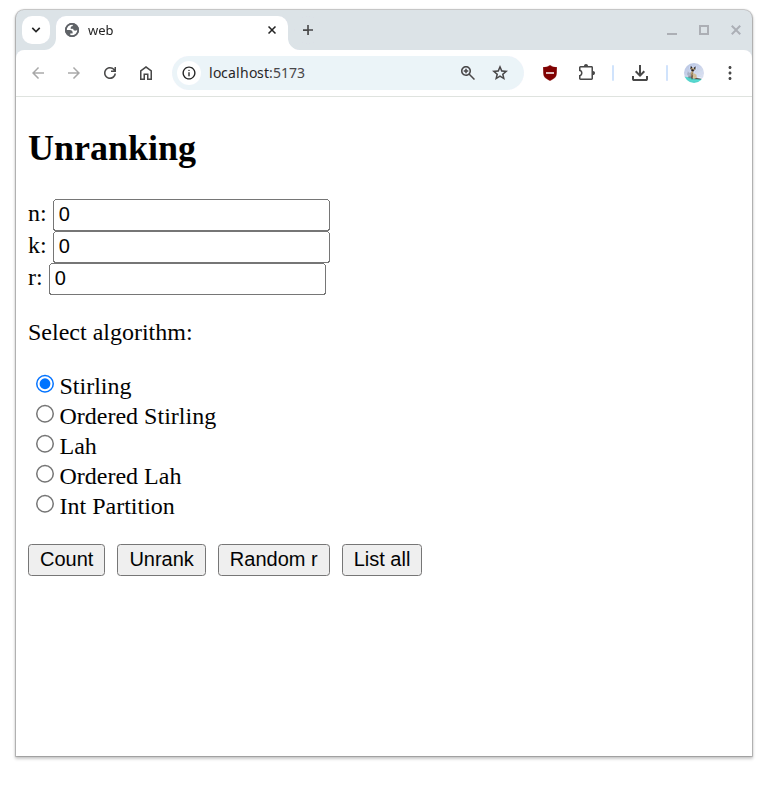
\includegraphics[width=0.75\textwidth]{images/webapp_main.png}
  \caption{Interface principale de l'application}
  \label{fig:webapp_main}
\end{figure}

Le bouton \textbf{Unrank} retourne la structure combinatoire correspondant au
rang $r$ donn\'e. Le bouton \textbf{Count} affiche le nombre total de structures
pour les param\`etres choisis. Le bouton \textbf{Random~r} tire un rang al\'eatoire
uniform\'ement dans $\{0, \ldots, \text{count}(n,k)-1\}$ et affiche la structure
correspondante, en mettant \`a jour le champ $r$ pour permettre la reproduction
du r\'esultat.

\begin{figure}[h]
  \centering
  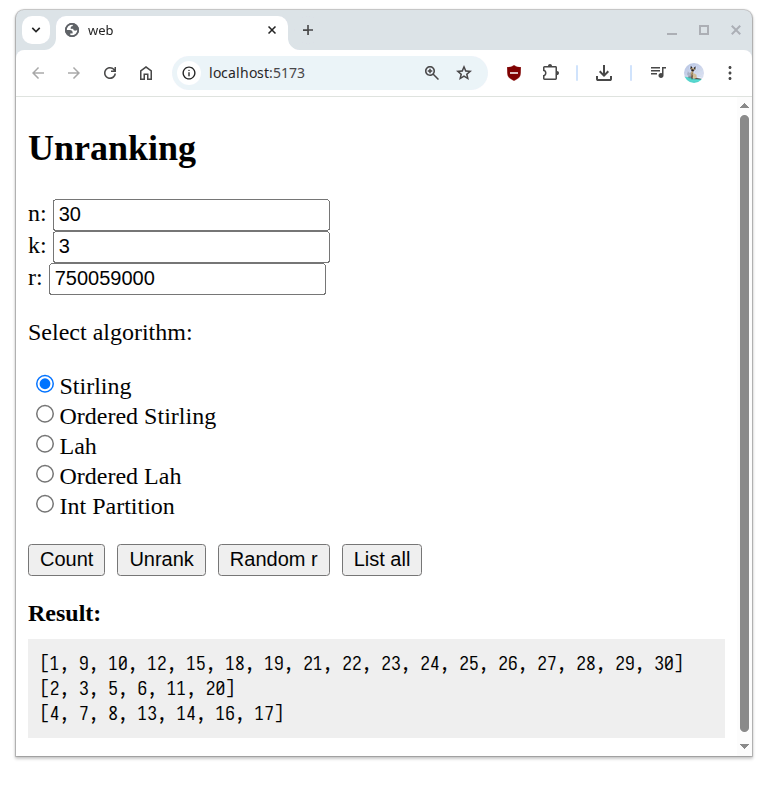
\includegraphics[width=0.75\textwidth]{images/webapp_unrank.png}
  \caption{R\'esultat d'un unranking pour les partitions de Stirling}
  \label{fig:webapp_unrank}
\end{figure}

Le bouton \textbf{List all} \'enum\`ere toutes les structures dans l'ordre
lexicographique, limit\'e \`a 1000 entr\'ees pour \'eviter de saturer
l'interface. Le nombre total est toujours affich\'e, et un avertissement
signale si la liste est tronqu\'ee.

\begin{figure}[h]
  \centering
  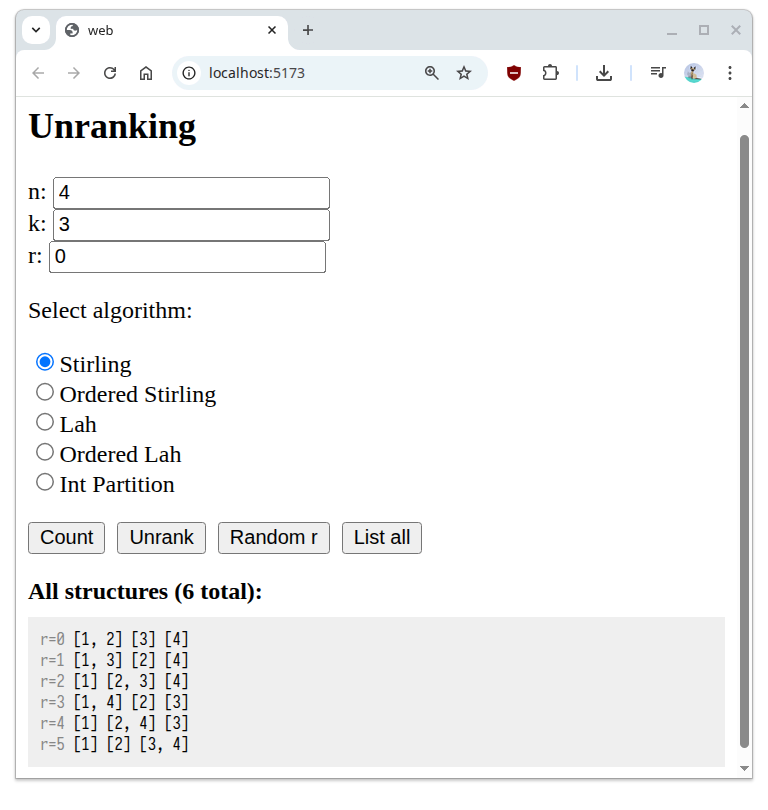
\includegraphics[width=0.75\textwidth]{images/webapp_listall.png}
  \caption{Liste des structures pour de petites valeurs de $n$ et $k$}
  \label{fig:webapp_listall}
\end{figure}

Enfin, lorsqu'un calcul est en cours, un bouton \textbf{Abort} appara\^it,
permettant d'interrompre le worker et d'en recr\'eer un nouveau sans recharger
la page.

\begin{figure}[h]
  \centering
  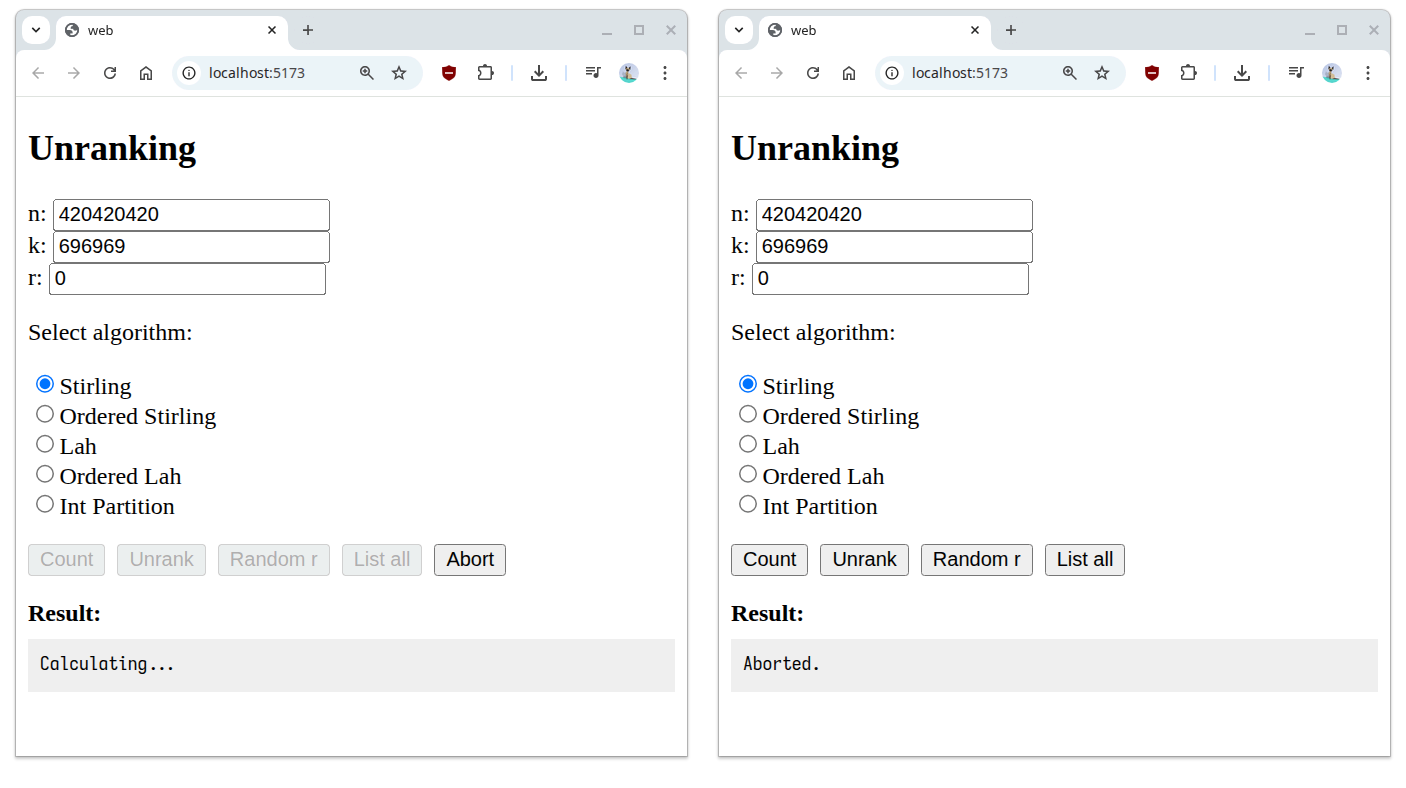
\includegraphics[width=1\textwidth]{images/webapp_abort.png}
  \caption{Bouton Abort visible pendant un calcul long}
  \label{fig:webapp_abort}
\end{figure}

\end{document}
